% System overview of the Nordhjem store (phases 1 to 3).
% Build: tectonic --outdir . fig-overview-v2.tex
\documentclass[border=16pt]{standalone}
\usepackage[T1]{fontenc}
\usepackage[utf8]{inputenc}
\usepackage{helvet}
\renewcommand{\familydefault}{\sfdefault}
\usepackage{tikz}
\usetikzlibrary{arrows.meta,positioning,calc}

\definecolor{ink}{HTML}{0F2A33}
\definecolor{muted}{HTML}{5E7078}
\definecolor{line}{HTML}{C3CED2}
\definecolor{blue}{HTML}{1F5FA8}
\definecolor{orange}{HTML}{E2551F}
\definecolor{hubfill}{HTML}{EDF2F4}
\definecolor{hubline}{HTML}{8FA3AC}

\newcommand{\lbl}[2]{\textbf{#1}\\[1.5pt]{\footnotesize\color{muted}#2}}

\begin{document}
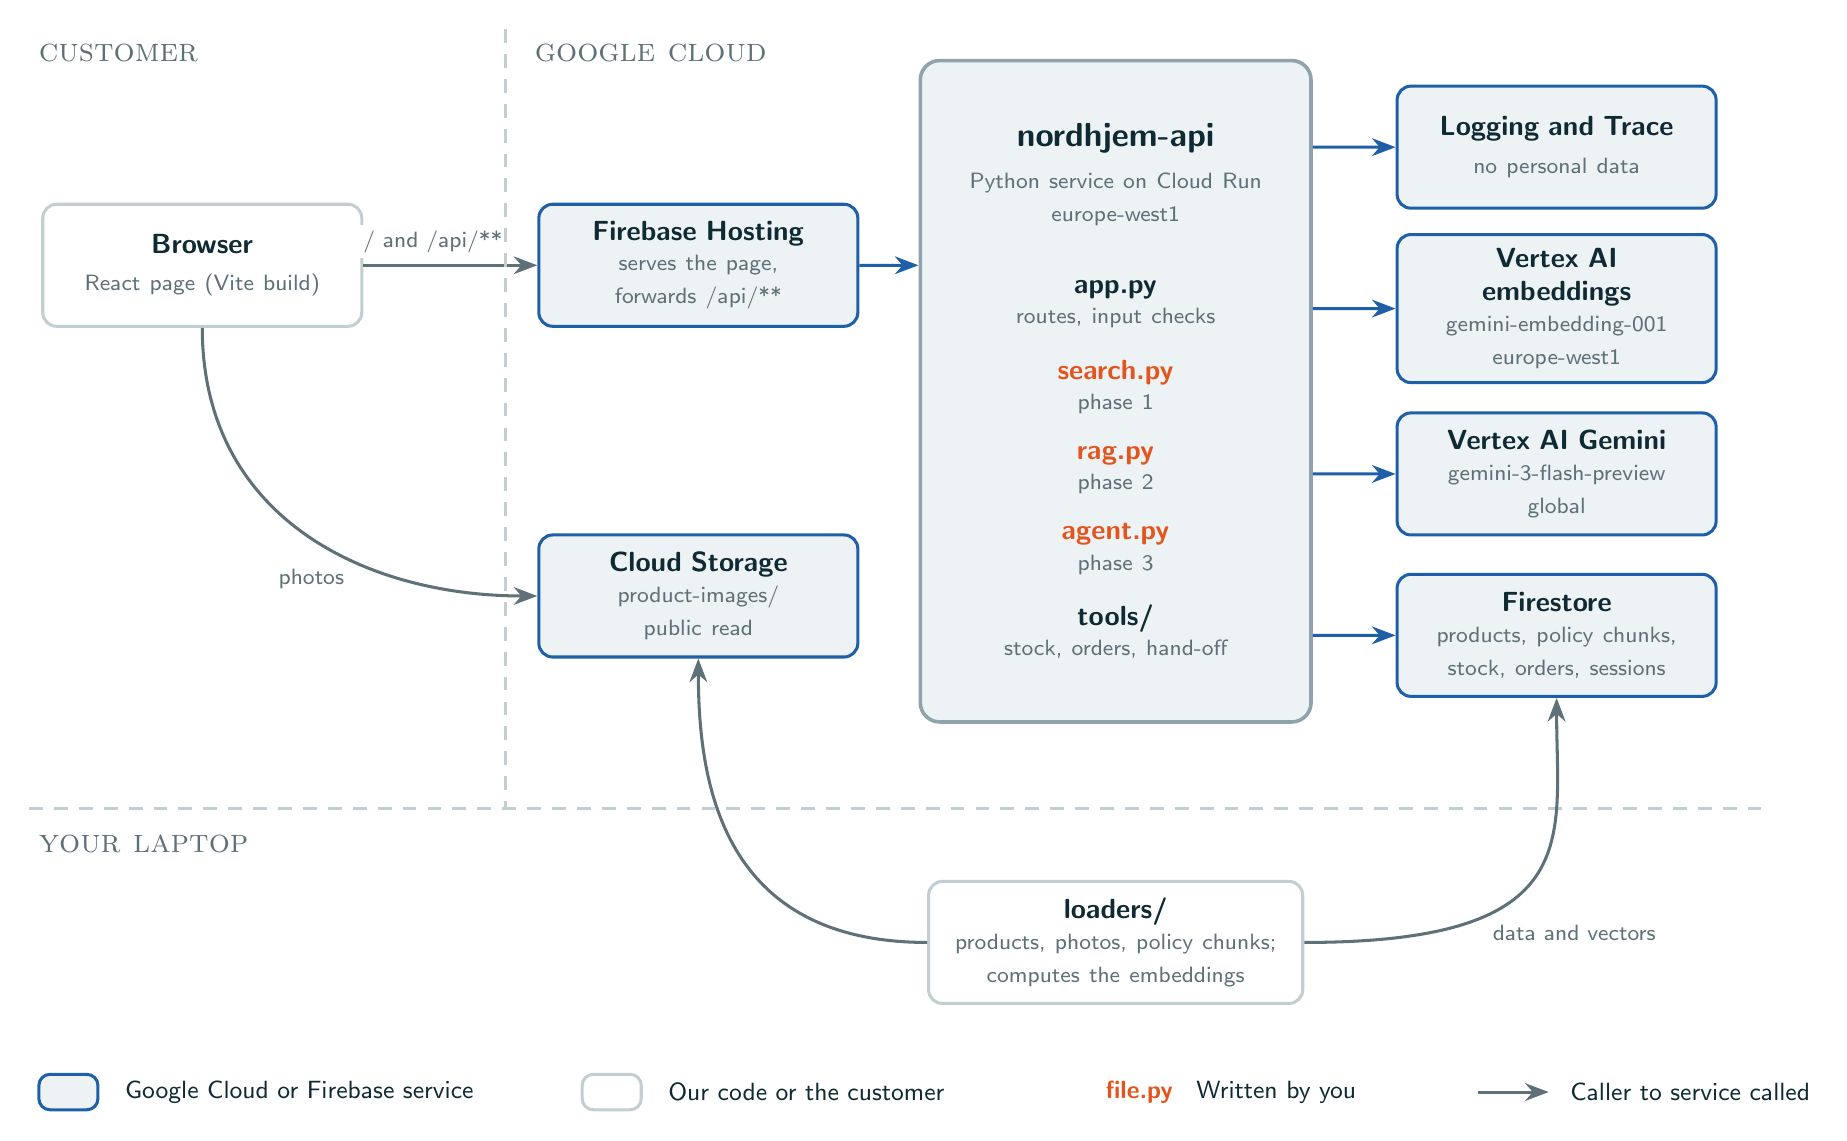
\begin{tikzpicture}[
  font=\sffamily,
  box/.style={rounded corners=5pt, draw=line, line width=1.1pt, fill=white,
    text=ink, align=center, text width=3.7cm, minimum height=1.55cm,
    inner sep=5pt},
  gcp/.style={box, draw=blue, fill=hubfill},
  one/.style={line width=1.1pt, draw=muted, -{Stealth[length=3mm]}},
  bone/.style={one, draw=blue},
  zone/.style={text=muted, font=\large\sffamily},
  note/.style={text=muted, font=\footnotesize\sffamily, fill=white,
    inner sep=2pt},
]

% ---- The API service: everything converges here ----
\node[rounded corners=7pt, draw=hubline, line width=1.3pt, fill=hubfill,
      text=ink, align=center, text width=4.4cm, minimum height=8.4cm,
      inner sep=8pt] (hub) at (0,0)
  {
   \textbf{\large nordhjem-api}\\[3pt]
   {\footnotesize\color{muted}Python service on Cloud Run}\\
   {\footnotesize\color{muted}europe-west1}\\[14pt]
   \textbf{app.py}\\[-1pt]{\footnotesize\color{muted}routes, input checks}\\[8pt]
   {\color{orange}\textbf{search.py}}\\[-1pt]
   {\footnotesize\color{muted}phase 1}\\[6pt]
   {\color{orange}\textbf{rag.py}}\\[-1pt]
   {\footnotesize\color{muted}phase 2}\\[6pt]
   {\color{orange}\textbf{agent.py}}\\[-1pt]
   {\footnotesize\color{muted}phase 3}\\[8pt]
   \textbf{tools/}\\[-1pt]
   {\footnotesize\color{muted}stock, orders, hand-off}};

% ---- Left: the customer side ----
\node[box] (browser) at (-11.6, 1.6)
  {\lbl{Browser}{React page (Vite build)}};
\node[gcp] (hosting) at (-5.3, 1.6)
  {\lbl{Firebase Hosting}{serves the page,\\forwards /api/**}};
\node[gcp] (storage) at (-5.3, -2.6)
  {\lbl{Cloud Storage}{product-images/\\public read}};

% ---- Right: data and models ----
\node[gcp] (firestore) at (5.6, -3.1)
  {\lbl{Firestore}{products, policy chunks,\\stock, orders, sessions}};
\node[gcp] (embed) at (5.6, 1.05)
  {\lbl{Vertex AI\\embeddings}{gemini-embedding-001\\europe-west1}};
\node[gcp] (gemini) at (5.6, -1.05)
  {\lbl{Vertex AI Gemini}{gemini-3-flash-preview\\global}};
\node[gcp] (logs) at (5.6, 3.1)
  {\lbl{Logging and Trace}{no personal data}};

% ---- Customer flows ----
\draw[one] (browser.east) -- node[note, pos=0.4, above=2pt] {/ and /api/**}
  (hosting.west);
\draw[bone] (hosting.east) -- ([yshift=1.6cm]hub.west);
\draw[one] (browser.south) .. controls +(0,-2.4) and +(-2.2,0)
  .. node[note, pos=0.62, below left=1pt] {photos} (storage.west);

% ---- Service flows ----
\draw[bone] ([yshift= 3.1cm]hub.east) .. controls +(1.4,0) and +(-1.4,0)
  .. (logs.west);
\draw[bone] ([yshift= 1.05cm]hub.east) -- (embed.west);
\draw[bone] ([yshift=-1.05cm]hub.east) -- (gemini.west);
\draw[bone] ([yshift=-3.1cm]hub.east) .. controls +(1.4,0) and +(-1.4,0)
  .. (firestore.west);

% ---- Laptop zone ----
\draw[line width=1pt, draw=line, dashed, dash pattern=on 5pt off 4pt]
  (-13.8,-5.3) -- (8.2,-5.3);
\draw[line width=1pt, draw=line, dashed, dash pattern=on 5pt off 4pt]
  (-7.75,4.6) -- (-7.75,-5.3);
\node[zone, anchor=west] at (-13.8,4.3) {\scshape customer};
\node[zone, anchor=west] at (-7.5,4.3) {\scshape google cloud};
\node[zone, anchor=west] at (-13.8,-5.75) {\scshape your laptop};

\node[box, text width=4.4cm] (loaders) at (0,-7.0)
  {\lbl{loaders/}{products, photos, policy chunks;\\computes the embeddings}};
\draw[one] (loaders.west) .. controls +(-2.6,0) and +(0,-1.6)
  .. (storage.south);
\draw[one] (loaders.east) .. controls +(3.6,0) and +(0,-1.8)
  .. (firestore.south)
  node[note, pos=0.3, below right=1pt] {data and vectors};

% ---- Legend ----
\node[rounded corners=4pt, draw=blue, line width=1.1pt, fill=hubfill,
      minimum width=0.75cm, minimum height=0.45cm] (k1) at (-13.3,-8.9) {};
\node[anchor=west, text=ink, font=\small] at ([xshift=0.2cm]k1.east)
  {Google Cloud or Firebase service};
\node[rounded corners=4pt, draw=line, line width=1.1pt, fill=white,
      minimum width=0.75cm, minimum height=0.45cm] (k2) at (-6.4,-8.9) {};
\node[anchor=west, text=ink, font=\small] at ([xshift=0.2cm]k2.east)
  {Our code or the customer};
\node[text=orange, font=\small\bfseries] (k3) at (0.3,-8.9) {file.py};
\node[anchor=west, text=ink, font=\small] at ([xshift=0.05cm]k3.east)
  {Written by you};
\draw[one] (4.6,-8.9) -- (5.5,-8.9);
\node[anchor=west, text=ink, font=\small] at (5.65,-8.9)
  {Caller to service called};

\end{tikzpicture}
\end{document}
